
%---------------------------------
\subsubsection{What is the geoid?}
\index{general}{Geoid}


There is an infinity of equipotential surfaces of the gravitational potential $U$.
However, there is a particular surface on the Earth that is "easy" to locate: 
the mean sea level. This is a somewhat arbitrary choice  
but it makes sense because the oceans are made of water (!): 
the surface of a fluid in equilibrium must follow an equipotential.

\begin{center}
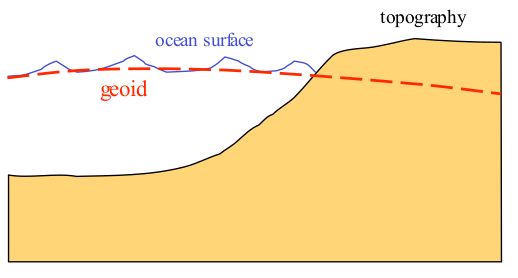
\includegraphics[width=6cm]{images/geoid/geoid1}
\end{center}

The geoid is usually defined in two ways:
\begin{itemize}
\item it is the particular equipotential surface that coincides with the mean sea level
 (easy to define in the oceans -assuming no currents, waves,... - but harder on land since 
it is not the topographic surface).
\item A gravitational equipotential surface. This means that everywhere at sea level experiences the same value of gravity potential, so there is no tendency for water to flow downhill since all points in the vicinity have the same value of gravity potential, pointed toward the center of the earth.
\end{itemize}

\begin{center}
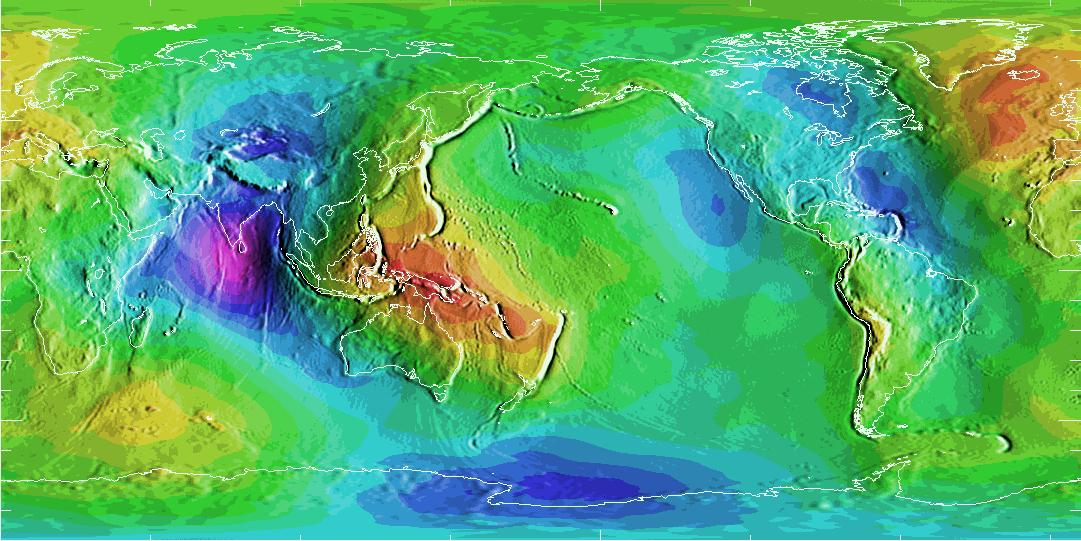
\includegraphics[width=10cm]{images/geoid/ww15mgh}\\
{\captionfont Data Max value: 85.4 meters, east of New Guinea. Data Min value:-107.0 meters, south of India. 
This image shows 15'x15' geoid undulations covering the planet Earth from the NIMA/GSFC WGS-84 EGM96 15' Geoid Height File. The undulations refer to the differences from the WGS-84(G873) reference ellipsoid. Map and description from National Geodetic Survey.}
\end{center}
%https://www.usna.edu/Users/oceano/pguth/md_help/geology_course/geoid.htm


%----------------------------------------
\subsubsection{the (reference) ellipsoid}

First evidence that the Earth is round Erathostene (275-195 B.C.)

First hypothesis that the Earth is flattened at the poles: Newton

First measurement of the Earth’s flattening at the poles: Clairaut (1736) and Bouguer (1743)

The shape of the Earth can be mathematically represented as an ellipsoid defined by:
\begin{itemize}
\item Semi-major axis = equatorial radius = $a$
\item Semi-minor axis = polar radius = $c$
\item Flattening (the relationship between equatorial and polar radius): $f = (a-c)/a$
\item Eccentricity: $e^2 =2f-f^2$
\end{itemize}

Many different reference ellipsoids have been defined and are in use.
We define the {\it reference ellipsoid} = the ellipsoid that best fits the geoid.
It is totally arbitrary, but practical. 
The most common reference ellipsoid is the WGS-84 one\footnote{\url{https://confluence.qps.nl/qinsy/latest/en/world-geodetic-system-1984-wgs84-182618391.html}}:

\begin{center}
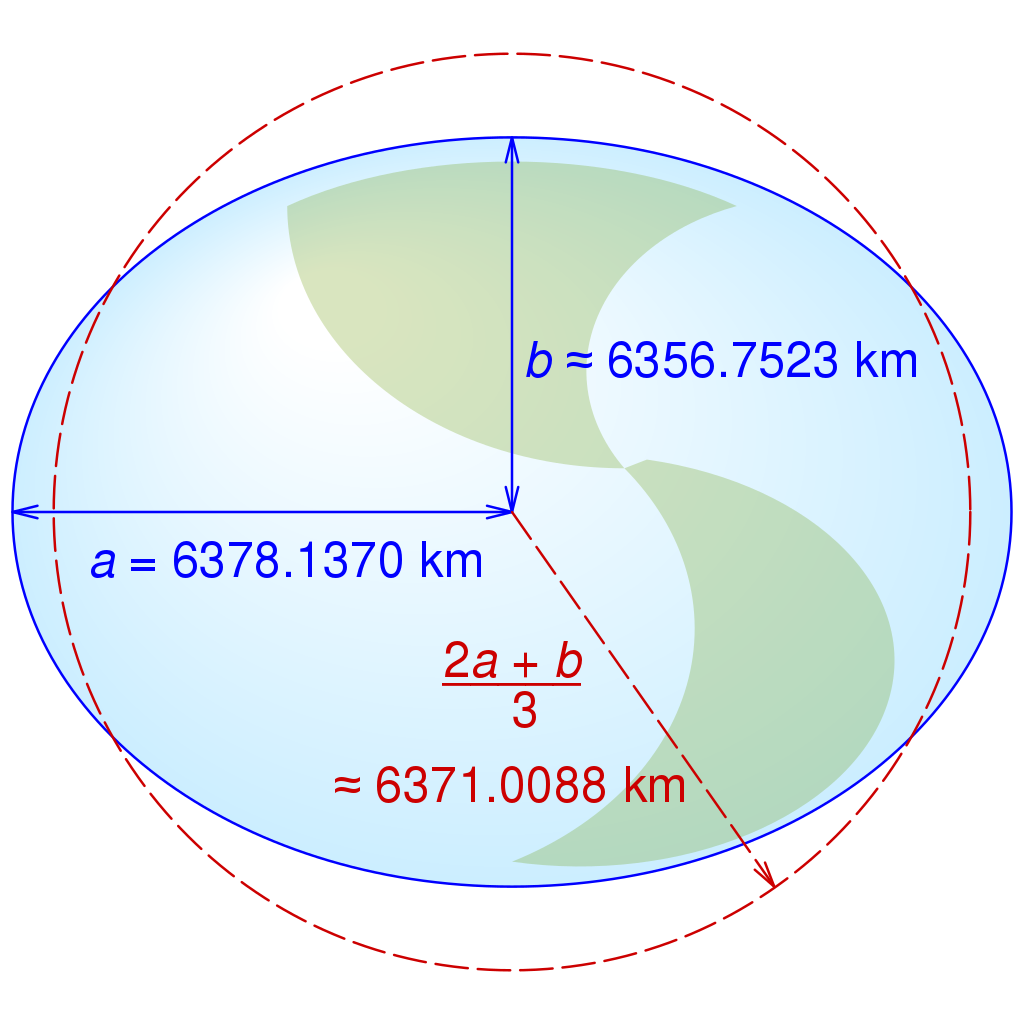
\includegraphics[width=6cm]{images/geoid/ellipsoid_wgs84}\\
Taken from \url{https://en.wikipedia.org/wiki/Reference_ellipsoid}
\end{center}


Geoid undulations = differences, in meters, between
the geoid reference ellipsoid
(= geoid “height”).

To clarify:
\begin{itemize}
\item Geoid = the equipotential surface of the Earth’s gravity field that
best fits (in a least squares sense) the mean sea level.
The gravitational potential is constant on the geoid (by definition) but 
the gravitational acceleration is not! 

\item Reference Ellipsoid = the ellipsoid that best fits the geoid 
\item Geoid = the (actual) figure of the Earth 
\item Ellipsoid = the (theoretical) shape of the Earth
\end{itemize}



%---------------------------------
\subsubsection{How to compute it?}

%---------------------------------
\subsubsection{Interesting modelling}

\begin{center}
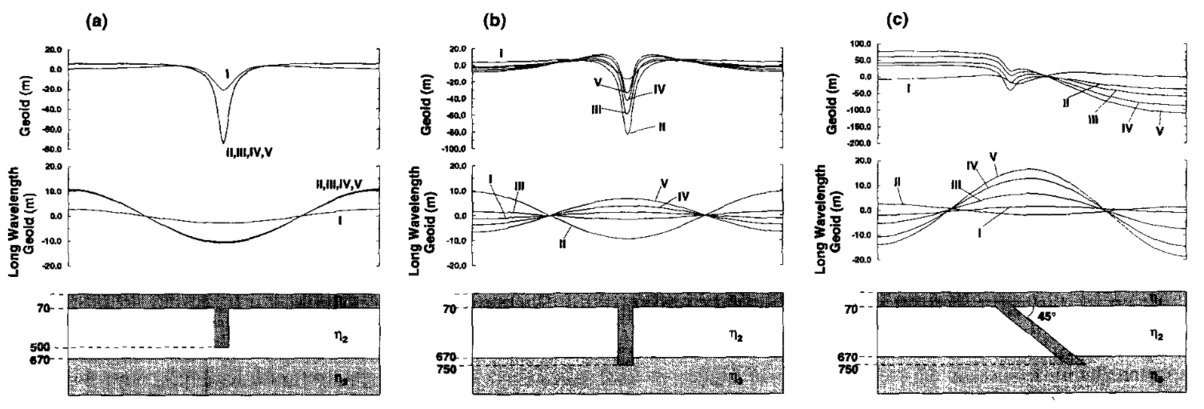
\includegraphics[width=15cm]{images/geoid/mogu96}
{\scriptsize Idealized 2D slab calculations for each viscosity model: geoid and geoid filtered 
to pass only the longest wavelengths ($\sim$ 4000 km).
(a) Cold slab extends to 500 km depth in the upper mantle, 
(b) Slab extends to 750 km so that it is partly supported by the high viscosity lower mantle at 670 km. 
(c) Slab tilted at 45\degree to the vertical extending to the top of the lower mantle. 
Taken from \cite{mogu96}}
\end{center}
